\chapter{Marco teórico}
\label{ch:marco}


En este cap\'itulo se detalla el contenido te\'orico necesario para el desarrollo de este trabajo. La propuesta consiste en la optimizaci\'on y paralelizaci\'on del filtro \engl{Deceived Non-Local Means} (DNLM). Este filtro es una modificaci\'on del filtro \engl{Non-Local Means} (NLM) que adiciona la mejora de bordes y contraste, conservando la preservaci\'on de bordes y la robustez ante el ruido proporcionada por el filtro NLM \cite{calderon2015dewaff}. 
Las optimizaciones computacionales del filtro NLM se pueden agrupar en dos enfoques: Optimizaciones exactas y aproximaciones del algoritmo. Existen propuestas de optimizaci\'on del rendimiento del filtro NLM en t\'erminos del ruido eliminado, sin embargo se emplean t\'ecnicas de cl\'ustering, diccionarios y otros m\'etodos probabil\'isticos para preclasificar parches similares en la imagen, a\~nadiendo complejidad computacional al procesamiento \cite{pardoNLM:2018,Chan2013,Tasdizen2009,Chatterjee2008,JI20091238,Karam2018}. 
La propuesta de paralelizaci\'on incluye la evaluaci\'on de dos optimizaciones computacionales exactas del filtro NLM adaptadas al filtro DNLM: DNLM-IIFFT y DNLM-MA.



\section{Eliminaci\'on de ruido}

\subsection{Ruido Blanco Aditivo de distribuci\'on Gaussiana}
\label{ch:marco_agwn}

El ruido presente en im\'agenes se debe a fen\'omenos naturales en el proceso de captura, transmisi\'on y almacenamiento de las im\'agenes. 	Una forma de modelar este ruido es mediante el ruido blanco aditivo de distribuci\'on gaussiana. Este ruido es llamado gaussiano porque se modela a trav\'es de una distribuci\'on de probabilidad gaussiana. Se dice que es blanco debido a que su espectro de intensidad es plano. Se le llama aditivo porque la distorci\'on causada por el ruido se modela a trav\'es de la suma del ruido a los pixeles de la imagen. El modelo de ruido gaussiano  est\'a dado por:

\begin{equation}
\label{eq:modelruido}
U = X + V \enspace ,
\end{equation}

 donde $U$ es la imagen con ruido gaussiano, $X$ corresponde a la imagen sin ruido y $V$ corresponde a una variable alatoria que sigue una funci\'on de densidad de probabilidad gaussiana dada por: 
 
\begin{equation}
\label{eq:probfuncgauus}
p(v(x)) = \frac{1}{{\sigma \sqrt {2\pi } }}e^{{{ - \left( {V(x) - \mu } \right)^2 } \mathord{\left/ {\vphantom {{ - \left( {x - \mu } \right)^2 } {2\sigma ^2 }}} \right. \kern-\nulldelimiterspace} {2\sigma ^2 }}} \enspace ,
\end{equation}

siendo $\sigma$ la desviaci\'on est\'andar  y $\mu$ el valor medio de la distribuci\'on de probabilidad, que para efectos del ruido gaussiano se asume $\mu = 0$.


\section{Filtro Non-Local Means}
\label{ch:marco_nlm}

El filtro NLM forma parte de los filtros espaciales de promedio ponderado que pueden definirse de manera general como:

\begin{equation}
\label{eq:weighted}
Y(U,p)=\left(\sum_{m\in \Omega}\psi\left(U, p, m\right)\right)^{-1} \\ \left(\sum_{m\in \Omega}\psi\left(U, p, m\right)U(m)\right) \enspace ,
\end{equation}

donde $p$ es el pixel que se pretende filtrar, $m$ corresponde a un pixel contenido en la ventana deslizante $\Omega$, $\psi$ es una funci\'on de pesado del filtro y $U$ la imagen de entrada \cite{calderon2015dewaff}.

La funci\'on de pesado del filtro NLM se define como:

\begin{equation}
\label{eq:nlmfunc}
\psi_{\textrm{NLM}}\left(U,p,m\right) = \exp\left(-\frac{\left\Vert \vec{\boldsymbol{\eta}}\left(m\right)-\vec{\boldsymbol{\eta}}\left(p\right)\right\Vert^2 }{\sigma^{2}}\right) \enspace ,
\end{equation}

donde $\sigma$ es el par\'ametro que controla el grado de suavizado del filtro y $\vec{\boldsymbol{\eta}}\left(q\right)$ el vector que contiene los pixeles de un vecindario con tama\~no $\omega$ al rededor de $q$, con $q \in \{p,m\}$.

Este filtro introduce el concepto de similitud entre vencindarios de pixeles y no entre sus intensidades, como en otros filtros. La funci\'on de pesado definida en (\ref{eq:nlmfunc}) hace uso de la distancia Euclidiana para determinar la similitud entre los vecindarios de los pixeles $p$ y $m$. 
De esta manera se determina el peso en la contribuci\'on para el ponderamiento de los pixeles en una regi\'on limitada por una ventana $\Omega$. Este enfoque reduce los cambios bruscos en la intensidad de pixeles aleda\~nos al comparar los vecindarios en un \'area local, a la vez que permite conservar detalles como bordes y patrones en la imagen\cite{calderon2015dewaff}. 


En cuanto a la complejidad computacional, al filtrar una imagen de entrada en escala de grises de $N$ pixeles, con una ventana deslizante de tama\~no $|\Omega| = S$ pixeles y un vecindario de tama\~no $|\omega| = P$ pixeles, la complejidad computacional del filtro DNLM es de $\mathcal{O}(N\cdot~S\cdot~P)$. 



\section{Mejora de bordes y contraste}

\subsection{Unsharp Masking}
\label{ch:marco_usm}

Los m\'etodos de Unsharp Masking se utilizan para el realce de los bordes y la mejora de contraste en las im\'agenes. Se realiza mediante una substracci\'on de la imagen suavizada a la imagen original. Esto origina una imagen $B$ con las frecuencias altas de la imagen, es decir, los bordes y otros cambios de intensidad bruscos en los pixeles t\'ipicamente representados como detalles y ruido. 

Adicionalmente, se puede emplear un enfoque inverso que consiste en sumar la imagen $B$ con la informaci\'on de bordes y detalles en alta frecuencia a la imagen original. La adici\'on se controla en una proporci\'on dada por el coeficiente $\lambda$, con:

\begin{equation}
\label{eq:unsharpmask}
G=U+\lambda~B \enspace .
\end{equation}

Por ejemplo, $B$ corresponde a

\begin{equation}
\label{eq:unsharfilter}
B=l*U \enspace 
\end{equation}

y $l$ puede estar dado por:

\begin{equation} l = \left[
\begin{array}{ccc}
1 & 1 & 1\\
1 & -8 & 1\\
1 & 1 & 1
\end{array}\right]
\end{equation}

para el caso de la aproximaci\'on al laplaciano.

La imagen $B$ se obtiene por medio de la convoluci\'on entre la imagen original y un kernel de aproximaci\'on al laplaciano, laplaciano de gaussiano o de diferencia de gaussianas.


En este trabajo se utiliza un kernel de aproximaci\'on al laplaciano por medio del laplaciano de gaussiano \cite{sotak1989laplacian}:

\begin{equation}
\label{eq:log}
\operatorname{LoG}(x,y) = \frac{1}{\pi\sigma^4}\left(\frac{x^2+y^2}{2\sigma^2} - 1\right)e^{-\frac{x^2+y^2}{2\sigma^2}},
\end{equation}

La figura \ref{fig:exampleUSM} muestra el resultado de aproximar al laplaciano de una de imagen de entrada y la salida del m\'etodo USM con la imagen mejorada en contraste y bordes. 

\begin{figure}[H]
%
\begin{minipage}{0.25\textwidth}
  \centering
  \centerline{
\includegraphics[width=\linewidth]{lena}}
%  \vspace{1.5cm}
  \centerline{(a) Imagen de entrada $U$.}\medskip
\end{minipage}
\hfill
\begin{minipage}{0.25\textwidth}
  \centering
  \centerline{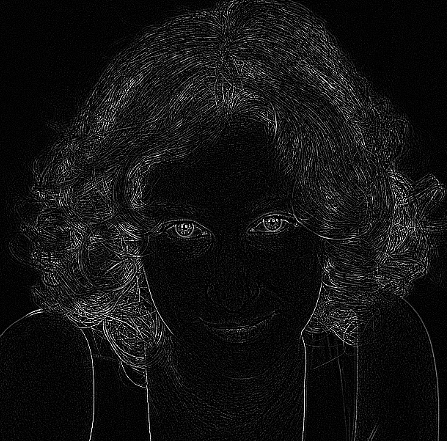
\includegraphics[width=\linewidth]{lena_lapl}}
%  \vspace{1.5cm}
  \centerline{(b) Laplaciano de $U$.}
\end{minipage}
\hfill
\begin{minipage}{0.25\textwidth}
  \centering
  \centerline{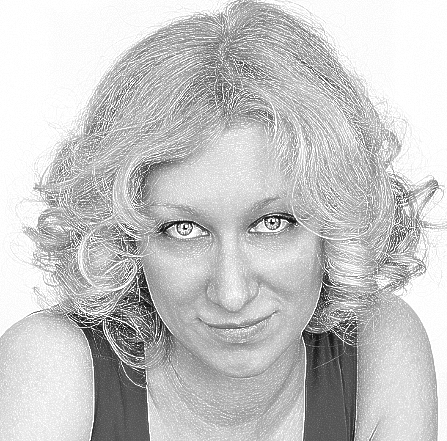
\includegraphics[width=\linewidth]{lena_sharp}}
%  \vspace{1.5cm}
  \centerline{(c) Imagen de salida $U_{\textrm{USM}}$.}\medskip
\end{minipage}
%
\caption[Ejemplo de mejora en imagen con \engl{Unsharp Mask}]{Salida del filtro USM con $\lambda = 5$ y $\sigma = 0.01$. \label{fig:exampleUSM}}
%
\end{figure}


\section{Filtro Deceived Non-Local Means}
\label{ch:marco_dnlm}


El enfoque del filtro \engl{Deceived Non-Local Means} (DNLM) consiste en la combinaci\'on de un m\'etodo de \engl{Unsharp Masking} (USM) con el filtro NLM, con el prop\'osito de lograr por un lado una mejora en los bordes y en el contraste de la imagen, y por otro lado la eliminaci\'on del ruido gausiano  presente en la imagen. La combinaci\'on propuesta se basa en el desacople entre la imagen usada en el pesado (imagen original $U$) y la utilizada en el filtrado $U_{\textrm{USM}}$. Esto permite evitar el efecto anillo presente en las im\'agenes filtradas con el USM \cite{calderon2015dewaff}.

La funci\'on del filtro DNLM est\'a dada por:

\begin{equation}
\label{eq:dnlm}
Y(U,p)=\left(\sum_{m\in \Omega}\psi_{NLM}\left(U, p, m\right)\right)^{-1} \\ \left(\sum_{m\in \Omega}\psi_{\textrm{NLM}}\left(U, p, m\right)U_{\textrm{USM}}(m)\right) \enspace ,
\end{equation}

donde $U$ es la imagen de entrada, $p$ es el pixel que se pretende filtrar, $m$ corresponde a un pixel contenido en la ventana deslizante $\Omega$, $\psi_{\textrm{NLM}}$ es una funci\'on de pesado del filtro NLM y $U_{\textrm{USM}}$ la imagen producto de la mejora con el m\'etodo USM \cite{calderon2015dewaff}. El desacople mostrado en (\ref{eq:dnlm}) se da al realizar el c\'alculo de los pesos con la imagen de entrada $U$ y el filtrado con la imagen $U_{\textrm{USM}$.

La figura \ref{fig:exampleDNLM} muestra el aumento en contraste de la imagen y el mayor detalle en bordes resultado del procesamiento con el filtro DNLM.

\begin{figure}[H]
\centering
\begin{minipage}[b]{0.3\textwidth}
  \centering
  \centerline{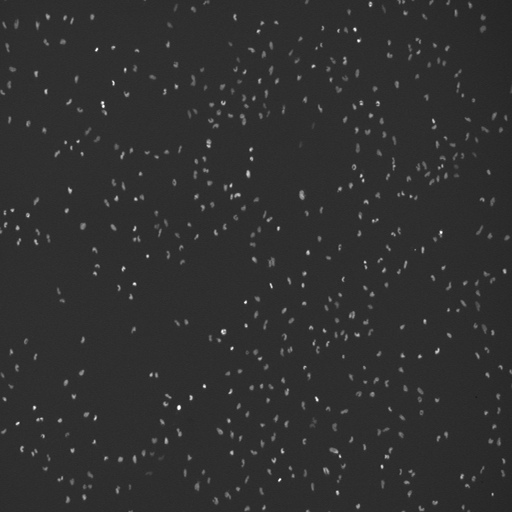
\includegraphics[width=\linewidth]{512x512}}
%  \vspace{1.5cm}
  \centerline{(a) Ejemplo de imagen de actividad celular.}\medskip
\end{minipage}
\hfill
\begin{minipage}[b]{0.3\textwidth}
  \centering
  \centerline{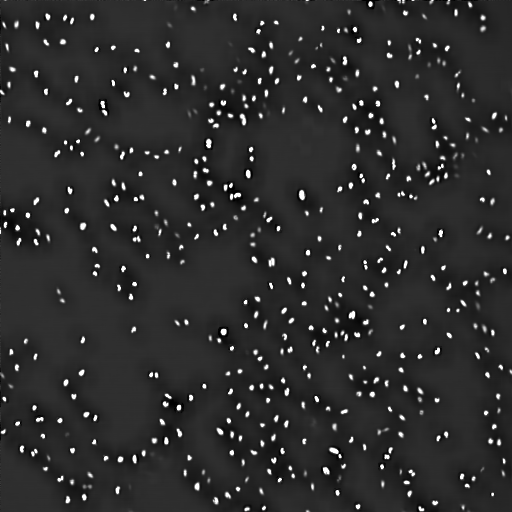
\includegraphics[width=\linewidth]{512x512_DeNLM}}
%  \vspace{1.5cm}
  \centerline{(b) Imagen fitrada.}
\end{minipage}
\vfill
\begin{minipage}[b]{0.3\textwidth}
  \centering
  \centerline{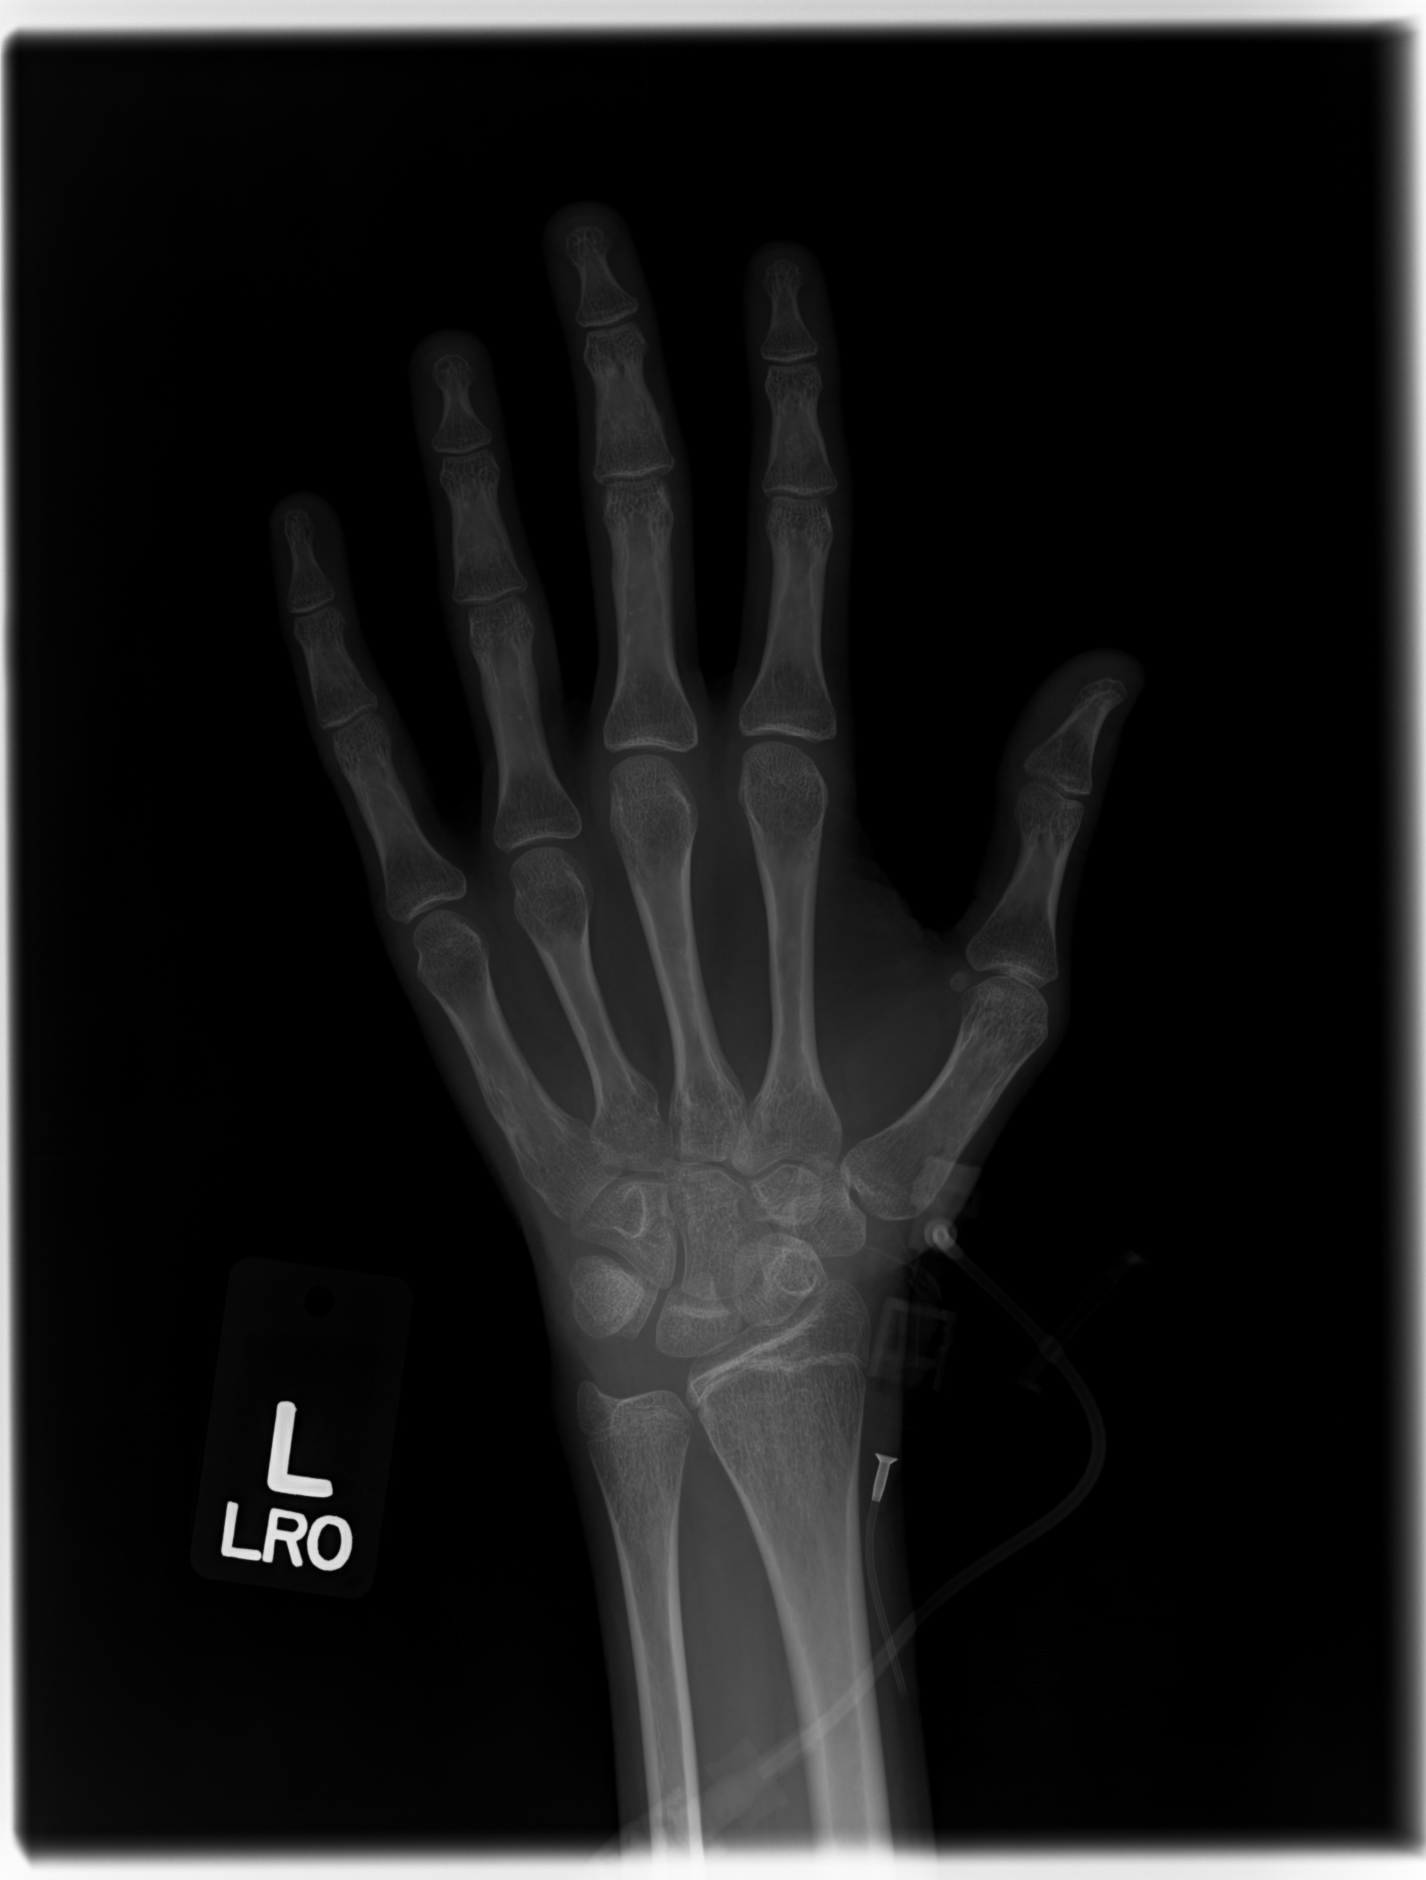
\includegraphics[width=\linewidth]{11043}}
%  \vspace{1.5cm}
  \centerline{(c) Imagen de rayos-x.}\medskip
\end{minipage}
\hfill
\begin{minipage}[b]{0.3\textwidth}
  \centering
  \centerline{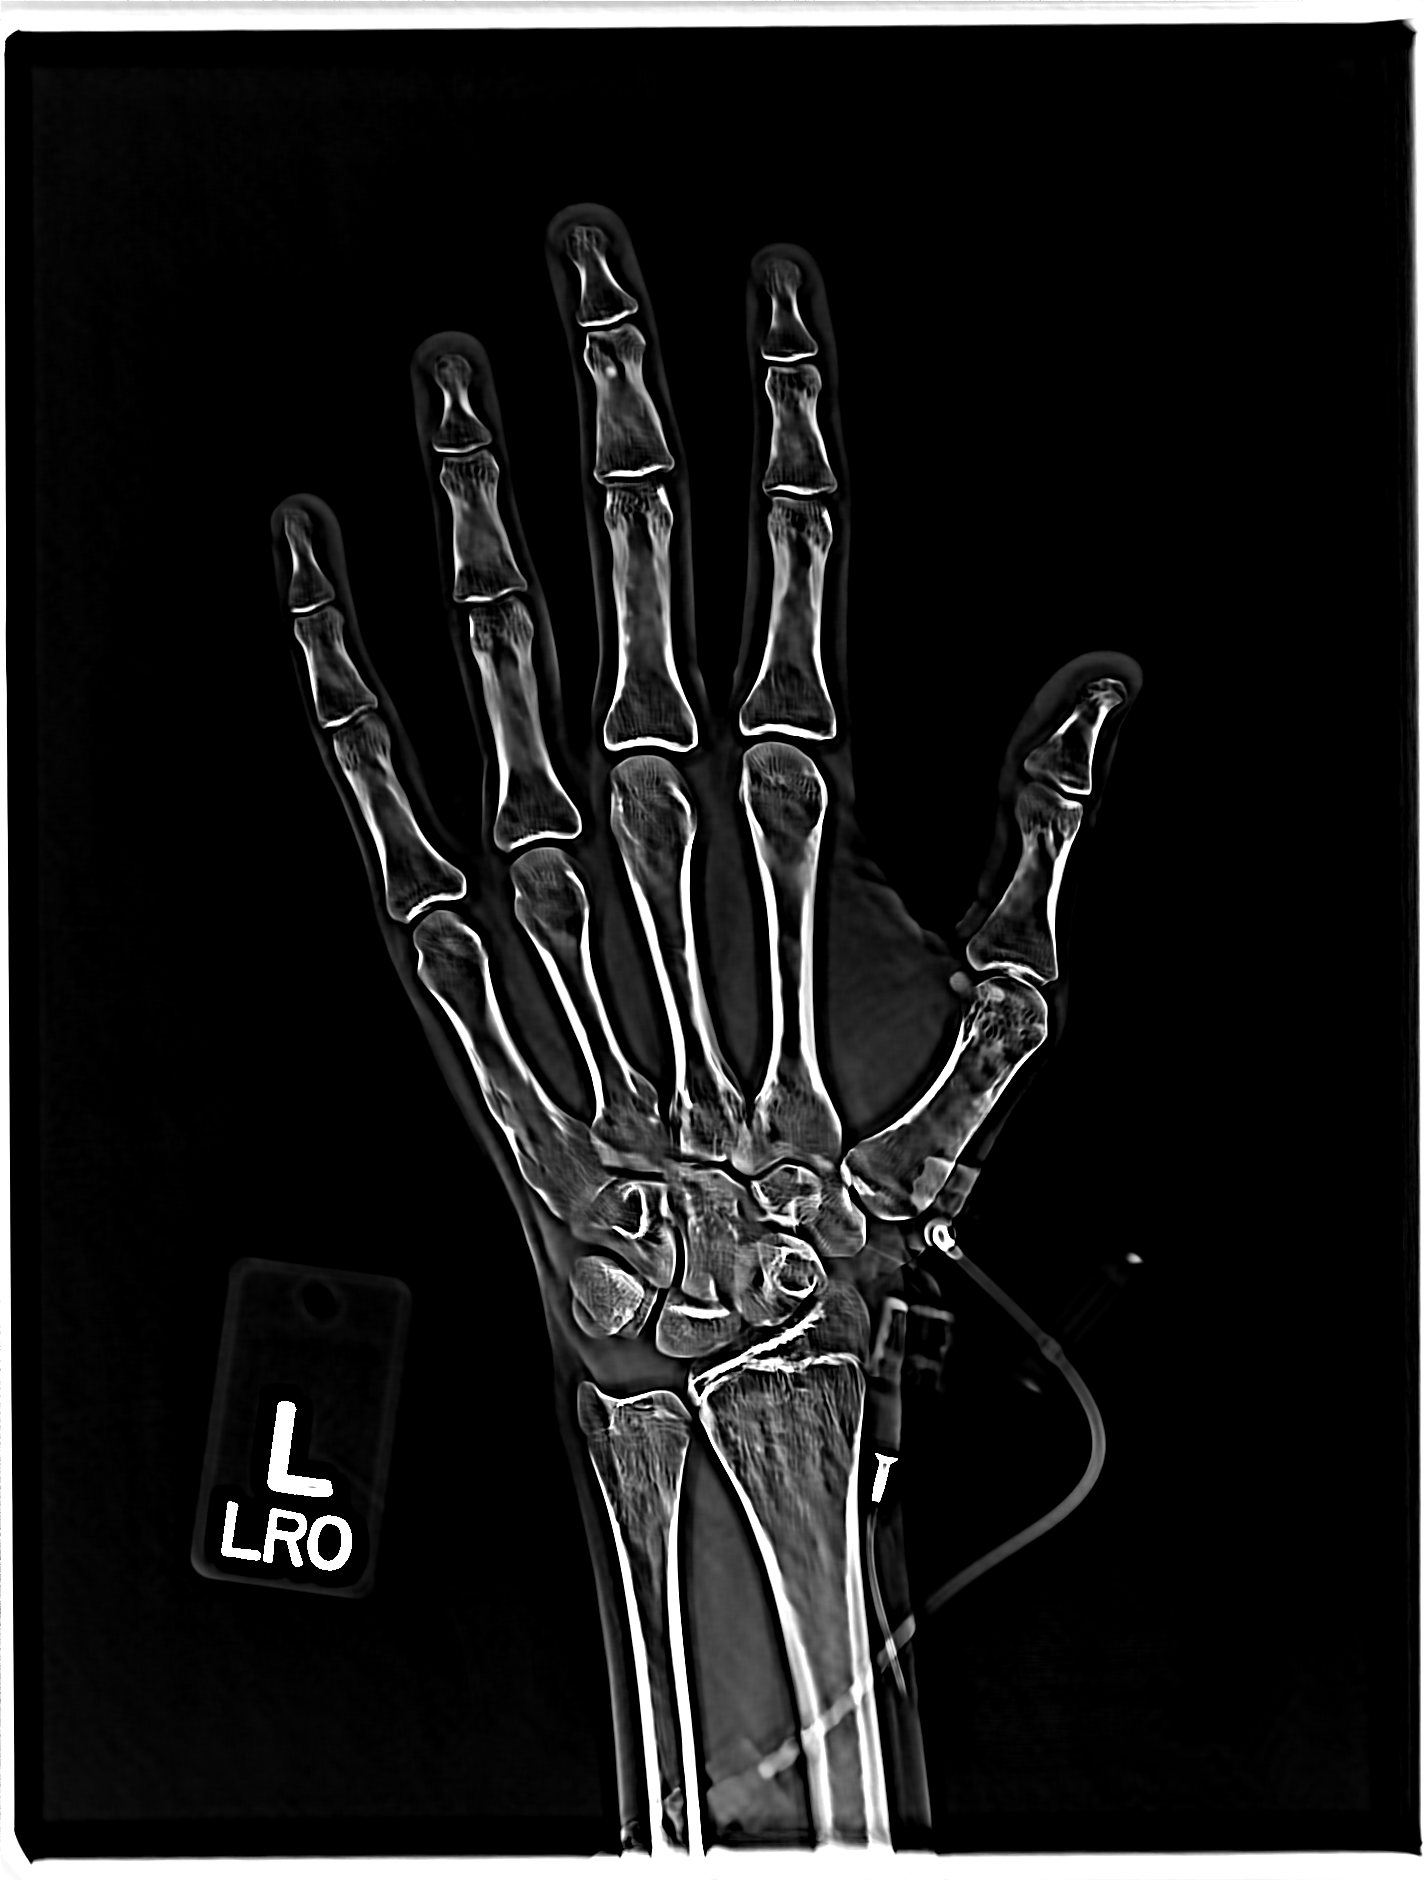
\includegraphics[width=\linewidth]{11043_DeNLM}}
%  \vspace{1.5cm}
  \centerline{(d) Imagen filtrada.}\medskip
\end{minipage}
%
\caption[Ejemplo de im\'agenes filtradas con el filtro DNLM]{Ejemplo de im\'agenes filtradas con el filtro DNLM. \label{fig:exampleDNLM}}

%
\end{figure}



\section{Optimizaciones computacionales}
\label{ch:marco_opt}

\subsection{DNLM-IIFFT}
\label{ch:marco_dnlmifft}

Esta optimizaci\'on computacional utiliza im\'agenes integrales y la transformada r\'apida de Fourier para disminuir la complejidad computacional del filtro DNLM. 



Al analizar la distancia euclidiana $D$ entre los vecindarios se tiene que:

\begin{equation}
D\left(x,y\right)=\left\Vert \vec{\boldsymbol{\eta}}\left(y\right)-\vec{\boldsymbol{\eta}}\left(x\right)\right\Vert^2 \enspace . 
\end{equation}

La ecuaci\'on anterior puede representarse en notacion matricial con la norma de Frobenius $\Vert \cdot \Vert_{F}$ como:


\begin{equation}
D\left(x,y\right)=\Vert \mat{Y} - \mat{X} \Vert_{F}^2 \enspace ,
\label{eq:distMat}
\end{equation}

con \mat{Y} y \mat{X} las matrices de los vecindarios de los pixeles $y$ y $x$. respectivamente.

Si se se define la norma $\Vert \cdot \Vert_{F}^2$ con el producto interno de Frobenius $\langle\,,\rangle_{F}$ se tiene que:

\begin{equation}\label{eq:frobProd}
\begin{split}
\Vert \mat{Y} - \mat{X} \Vert_{F}^2 & = \langle\mat{Y} - \mat{X},\mat{Y} - \mat{X}\rangle_{F}  \quad \text{y por sesquilinealidad:}\\ 
& = \langle\mat{Y},\mat{Y}\rangle_{F} + \langle\mat{Y},-\mat{X}\rangle_{F} + \langle-\mat{X},\mat{Y}\rangle_{F} + \langle-\mat{X},-\mat{X}\rangle_{F}\\
& = \Vert \mat{Y} \Vert_{F}^2 -2\langle\mat{Y},\mat{X}\rangle_{F} + \Vert \mat{X} \Vert_{F}^2 \enspace ,
\end{split} 
\end{equation}


tomando en cuenta que $\Vert \cdot \Vert_{F}^2$ es una norma que cumple todos los axiomas correspondientes. 

\begin{table}
\begin{center}
\caption{Ejemplo de imagen de entrada \mat{U}.\label{table:imageExample}}

\renewcommand{\arraystretch}{1.4}
\setlength\tabcolsep{3pt}

{
\begin{tabular}{cc|ccc|c}
 & \multicolumn{1}{c}{\textbf{1}} & \textbf{2} & \textbf{3} & \multicolumn{1}{c}{\textbf{4}} & \textbf{5}\tabularnewline
\textbf{1} & \multicolumn{1}{c}{5} & 12 & 1 & \multicolumn{1}{c}{3} & 2\tabularnewline
\cline{3-5} 
\textbf{2} & 5 & 2 & 3 & 1 & 4\tabularnewline
\textbf{3} & 3 & 1 & \textbf{2} & 3 & 1\tabularnewline
\textbf{4} & 4 & 3 & 2 & 1 & 3\tabularnewline
\cline{3-5} 
\textbf{5} & \multicolumn{1}{c}{1} & 5 & 6 & \multicolumn{1}{c}{5} & 3\tabularnewline
\end{tabular}
}
\par\end{center} 
\end{table}

El siguiente ejemplo ilustra el c\'alculo de la norma de Frobenius entre los vecindarios de pixeles contenidos en la imagen $\mat{U} \in\mathbb{R}^{5 \times 5}$ definida en la Tabla \ref{table:imageExample}. Para efectos de la ilustraci\'on, se toman los vecindarios $\mat{P}_{\left(3,3\right)},\mat{P}_{\left(2,2\right)} \in\mathbb{R}^{3\times3}$ de la imagen de ejemplo \mat{U}  y se realiza  el c\'alculo de la norma de Frobenius tal que:


\begin{equation}
\label{eq:resultado1}
\begin{split}
\left\Vert \mat{P}_{\left(3,3\right)}-\mat{P}_{\left(2,2\right)}\right\Vert_{F} ^{2} & =\left\Vert \left[\begin{array}{ccc}
2 & 3 & 1\\
1 & 2 & 3\\
3 & 2 & 1
\end{array} \right]-\left[\begin{array}{ccc}
5 & 12 & 1\\
5 & 2 & 3\\
3 & 1 & 2
\end{array}\right]\right\Vert_{F}^2 \\
& =\left\Vert\left[\begin{array}{ccc}
-3 & -9 & 0\\
-4 & 0 & 0\\
0 & 1 & -1
\end{array}\right]\right\Vert_{F}^2 \\
& =108 \enspace .
\end{split}
\end{equation}



Al desarrollar (\ref{eq:resultado1}) como se muestra en (\ref{eq:frobProd}), se obtiene que: 
\begin{equation}\label{eq:matFrodProd}
\resizebox{.9 \textwidth}{!} 
{
\begin{split}
\lVert \mat{P}_{\left(3,3\right)}-\mat{P}_{\left(2,2\right)}\rVert_{F} ^{2} & =\lVert \mat{P}_{\left(3,3\right)}\rVert_{F}^2 -2\langle\mat{P}_{\left(3,3\right)},\mat{P}_{\left(2,2\right)}\rangle_{F} + \lVert \mat{P}_{\left(2,2\right)}\rVert_{F}^2  \\
& = \left\Vert\left[\begin{array}{ccc}
2 & 3 & 1\\
1 & 2 & 3\\
3 & 2 & 1
\end{array}\right]\right\Vert_{F}^2-2\left\langle\left[\begin{array}{ccc}
2 & 3 & 1\\
1 & 2 & 3\\
3 & 2 & 1
\end{array}\right],\left[\begin{array}{ccc}
5 & 12 & 1\\
5 & 2 & 3\\
3 & 1 & 2
\end{array}\right]\right\rangle_{F}
+\left\Vert\left[\begin{array}{ccc}
5 & 12 & 1\\
5 & 2 & 3\\
3 & 1 & 2
\end{array}\right]\right\Vert_{F}^2 \\
& =42+-2\cdot78+222\\
& =42-156+222\\
& =108 \enspace ,
\end{split}
}
\end{equation}


consistente con los resultados obtenidos en (\ref{eq:resultado1}).




Esta optimizaci\'on del filtro DNLM se centra en el c\'alculo de la norma de Frobenius desarrollada en  (\ref{eq:frobProd}) de la siguiente manera:

\begin{itemize}
\item El uso de la imagen integral cuadr\'atica para calcular los t\'erminos $\Vert \mat{Y} \Vert_{F}^2 $ y $\Vert \mat{X} \Vert_{F}^2 $.
\item Calcular la convoluci\'on para obtener el t\'ermino $-2\langle\mat{Y},\mat{X}\rangle_{F} $
correspondiente a la correlaci\'on del vecindario \mat{Y} con la ventana de b\'usqueda \mat{\Omega}, para acceder posteriormente al $i$-\'esimo elemento del resultado.
\end{itemize}

Lo anterior permite disminuir la complejidad computacional del filtro a $O(S\log(S) \cdot N)$.
 
\subsubsection{Im\'agenes integrales}


La imagen integral $\mat{I}_{\Sigma}$ de una imagen de entrada \mat{U} presentada en \cite{viola2001robust}, est\'a dada por: 
\begin{equation}
\mat{I}_{\Sigma}\left(x,y\right)=\sum_{i\leq x}\sum_{j\leq y}u_{ij} \enspace ,
\end{equation}
la cual corresponde a la sumatoria de todos los  pixeles ubicados a la izquierda y superiores al pixel $u_{ij}$ de la imagen de entrada \mat{U}.

\begin{table}
\begin{center}
\caption{Ejemplo de imagen de entrada \mat{U^{\odot 2}}.\label{table:imageExample2}}

\renewcommand{\arraystretch}{1.4}
\setlength\tabcolsep{3pt}

{
\begin{tabular}{cc|ccc|c}
 & \multicolumn{1}{c}{\textbf{1}} & \textbf{2} & \textbf{3} & \multicolumn{1}{c}{\textbf{4}} & \textbf{5}\tabularnewline
\textbf{1} & \multicolumn{1}{c}{5} & 12 & 1 & \multicolumn{1}{c}{3} & 2\tabularnewline
\cline{3-5} 
\textbf{2} & 25 & 4 & 9 & 1 & 16\tabularnewline
\textbf{3} & 9 & 1 & \textbf{2} & 9 & 1\tabularnewline
\textbf{4} & 16 & 9 & 4 & 1 & 9\tabularnewline
\cline{3-5} 
\textbf{5} & \multicolumn{1}{c}{1} & 5 & 6 & \multicolumn{1}{c}{5} & 3\tabularnewline
\end{tabular}
}
\par\end{center} 
\end{table}


Continuando con el ejemplo previamente mostrado, la imagen de entrada \mat{U} con sus elementos elevados al cuadrado se define como el producto de Hadamard $\mat{U}^{\odot 2} = \mat{U} \odot \mat{U}$, como se muestra en la tabla \ref{table:imageExample2}. 


\begin{table}
\caption{Imagen integral para $U^{\odot2}$.\label{table:integralcuad}}
\begin{center}
\renewcommand{\arraystretch}{1.4}
\setlength\tabcolsep{3pt}
{
\begin{tabular}{cc|ccc|c}
 & \multicolumn{1}{c}{\textbf{1}} & \textbf{2} & \textbf{3} & \multicolumn{1}{c}{\textbf{4}} & \textbf{5}\tabularnewline
\textbf{1} & \multicolumn{1}{c}{\textbf{25(a)}} & 169 & 170 & \multicolumn{1}{c}{\textbf{179(b)}} & 183\tabularnewline
\cline{3-5} 
\textbf{2} & 50 & 198 & 208 & 218 & 238\tabularnewline
\textbf{3} & 59 & 208 & \textbf{222} & 241 & 262\tabularnewline
\textbf{4} & \textbf{75(c)} & 233 & 251 & \textbf{271(d)} & 301\tabularnewline
\cline{3-5} 
\textbf{5} & \multicolumn{1}{c}{76} & 259 & 313 & \multicolumn{1}{c}{358} & 397\tabularnewline
\end{tabular}
}
\par\end{center}
\end{table}


La imagen integral $\mat{I}_{\Sigma}$ se puede calcular iterativamente para un pixel espec\'ifico de la imagen de entrada \mat{U} de la siguiente manera: 
\begin{equation}
\mat{I}_{\Sigma}\left(x,y\right)=\mat{U}\left(x,y\right)-\mat{I}_{\Sigma}\left(x-1,y-1\right)+\mat{I}_{\Sigma}\left(x,y-1\right)
+\mat{I}_{\Sigma}\left(x-1,y\right) \enspace ,
\end{equation}

lo cual, para el ejemplo anterior significa que:

\begin{equation}
\mat{I}_{\Sigma}\left(3,3\right)=4-198+208+208=222 \enspace .
\end{equation}

Las im\'agenes integrales son \'utiles para calcular la sumatoria sobre una regi\'on determinada de la imagen, con una complejidad computacional constante de $\mathcal{O}(1)$. 

Al utilizar la imagen integral $\mat{I}_{\Sigma}$ para calcular la sumatoria de una regi\'on de la imagen original \mat{U}, limitada por los pixeles $a=\left(x_{0},y_{0}\right)$,
$b=\left(x_{1},y_{0}\right)$, $c=\left(x_{0},y_{1}\right)$ and $d=\left(x_{1},y_{1}\right)$, ilustrados en la Tabla \ref{table:integralcuad}, se calcula como: 

\begin{equation}
\sum_{i>x_{0}}^{i\leq x_{1}}~\sum_{j>y_{0}}^{j\leq y_{1}}u_{ij}=\mat{I}_{\Sigma}\left(d\right)+\mat{I}_{\Sigma}\left(a\right)-\mat{I}_{\Sigma}\left(b\right)-\mat{I}_{\Sigma}\left(c\right) \enspace ,
\end{equation}

y en el ejemplo presentado para una ventana de $3\times3$ pixeles alrededor del pixel $u_{3,3}^2$ de la imagen $\mat{U}^{\odot2}$ , los pixeles de las esquinas est\'an dados por: $a=\left(1,1\right)$, $b=\left(4,1\right)$,
$c=\left(1,4\right)$ y $d=\left(4,4\right)$, como se muestra en la Tabla \ref{table:imageExample2}. El c\'alculo de la sumatoria de los pixeles en la regi\'on especificada est\'a dada por: 

\begin{equation}
\sum_{i>1}^{i\leq 4}~\sum_{j>1}^{j\leq 4}u_{i,j}^2=271+25-179-75=42 \enspace ,
\end{equation}

lo cual, es consistente con el t\'ermino $\mat{P}_{\left(3,3\right)}$ en (\ref{eq:matFrodProd}). 



\subsubsection{Convoluci\'on y transformada r\'apida de Fourier}

Como se mostr\'o anteriormente, el t\'ermino $-2\langle\mat{Y},\mat{X}\rangle_{F}$ producto del desarrollo de la norma de Frobenius en (\ref{eq:matFrodProd}), puede representarse como el $i$-\'esimo elemento de la matriz resultante de la correlaci\'on del vecindario \mat{X} del pixel $x_{ij}$ con la ventana \mat{\Omega} como:

\begin{equation}
-2\langle\mat{Y},\mat{X}\rangle_{F} = -2\left[\mat{\Omega} \otimes \mat{X}\right](i,j) \enspace .
\end{equation}

Para expresar la correlaci\'on en t\'erminos de la convoluci\'on, se debe rotar la matriz \mat{X} de modo que se cumple que:

\begin{equation}
\mat{\Omega} \otimes \mat{X} = \mat{\Omega}*\mat{X}\mat{I}^T \enspace ,
\end{equation}

donde $\mat{I}^T$ es la matriz identidad transpuesta del vecindario \mat{X}. Lo anterior implica que el t\'ermino sea calculado como:

\begin{equation}
-2\langle\mat{Y},\mat{X}\rangle_{F} = -2\left[\mat{\Omega} *\mat{X}\mat{I}^T\right](i,j) \enspace .
\end{equation}




\subsection{DNLM-MA}
\label{ch:marco_condat}

Esta propuesta de optimizaci\'on computacional del filro NLM se caracteriza por su simpleza, al proponer un intercambio entre los ciclos de interaci\'on del algoritmo \cite{Condat2010}. La aceleraci\'on se consigue al incorporar simetr\'ia y convoluciones al realizar el ponderamiento de la reg\'on definida por la ventana de b\'usqueda \mat{\Omega}, para todos los pixeles la imagen de manera simult\'anea.

Siguiendo la definici\'on de la funci\'on de pesado del filtro NLM en (\ref{eq:nlmfunc}), un pixel $y$ puede ser expresado en t\'erminos del desplazamiento desde un pixel $x$ como $y = x + \Delta$. Por ejemplo, para una ventana de b\'usqueda $\vert\Omega\vert = 5 \times 5$, $\Delta$ puede tomar los valores $\Delta=0$, $\Delta=1$, $\Delta=2$ y en general, puede tomar valores de hasta $\Delta=\vert\Omega\vert/2$. Por lo tanto, la funci\'on de pesado del filtro NLM es sim\'etrica si:

\begin{equation}\
\psi_{\text{NLM}}(\mat{U}, x, x + \Delta) = \psi_{\text{NLM}}(\mat{U}, y, y - \Delta)  \enspace . 
\label{eq:symmetry}
\end{equation}

Los pesos son calculados al intercambiar los ciclos del algoritmo, ya que se itera sobre cada desplazamiento $\Delta$, en lugar de iterar sobre cada uno de los pixeles de la imagen de entrada. Para cada una de las iteraciones, la diferencia cuadr\'atica es calculada para toda la imagen como:

\begin{equation}
\mat{D}_\Delta\left(x\right) = \left(\mat{U}\left(x\right) - \mat{U}\left( x + \Delta \right)\right)^{\circ2}  \enspace ,
\label{eq:diffquad}
\end{equation}

donde la potencia al cuadrado es para cada pixel individual, siguiendo la notaci\'on de Hadamard. Seguidamente, se calcula la convoluci\'on de
$\mat{D}_\Delta$ con un kernel de promediado de tama\~no $\omega$ de la siguiente forma:
\begin{equation}
\label{eq:convmoas}
\mat{E}_{\Delta} = \mat{D}_{\Delta} * \mat{G} \enspace ,
\end{equation}

donde se define la convoluci\'on con un kernel $h$ (\ref{eq:convmoas}) que corresponde a un kernel de promediado.


El resultado es la funci\'on de pesado del filtro DNLM-MA: 

\begin{equation}
\psi_{DNLM-MA}=\exp^{\circ}\left(-\frac{ E_\Delta\left(x\right) }{h}\right)  \enspace .
\label{eq:wmoas}
\end{equation}


Con esto se consigue reducir la  funci\'on de costo computacional a $O(\sqrt{P} \cdot S \cdot N)$.  



\section{Arquitectura Intel Xeon Phi Knights Landing}
\label{ch:marco_xeonphi}

La arquitectura de procesador Intel Xeon Phi Knights Landing conocida como \textit{many-core} est\'a dise\~nada para aplicaciones de computaci\'on de alto rendimiento y es considerada la alternativa de Intel al desarrollo de algoritmos en GPU para prop\'osito general. A diferencia de la versi\'on anterior, esta nueva iteraci\'on con nombre clave Knights Landig permite el arranque de un sistema operativo por s\'i misma y provee m\'as de 3 TFLOP/s de precisi\'on doble y cerca de 6 TFLOP/s de precisi\'on doble \cite{Jeffers201663}. Posee de 32 a 36 celdas interconectadas por una interfaz de comunicaci\'on en 2D, cada una de ellas conformada por 2 CPU y 1MB de cach\'e L2 compartido \cite{XeonPhiWhitePaper}. Cada uno de los CPU incorpora 2 Unidades de Procesamiento Vectorial (VPU) con registros de hasta 512 bytes de largo, capaces de operar de manera simult\'anea para 2 o m\'as hilos \ref{XeonPhiWhitePaper}. 
Entre las caracter\'isticas que destacan del CPU es su modo de ejecuci\'on fuera de orden y el multihilo simult\'aneo de 4 hilos \cite{XeonPhiWhitePaper}. Una de sus particularidades es la incorporaci\'on de 16GB de Memoria de Alto Ancho de Banda (MCDRAM) de hasta $450 Gbyte/s$ en el mismo chip como lo muestra la Figura \ref{fig:cpu_phi}, permitiendo tiempos de latencia cortos en comparaci\'on con los obtenidos con tecnolog\'ias DDR4 \cite{XeonPhiWhitePaper}.

\begin{figure}
\centering
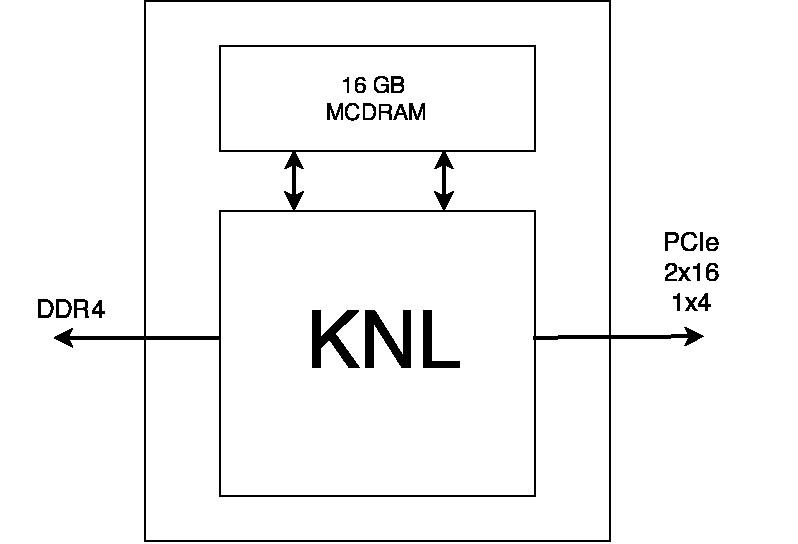
\includegraphics[width=0.5\textwidth]{fig/cpu}
\caption{Diagrama de alto nivel del procesador Xeon Phi KNL.}
\label{fig:cpu_phi}
\end{figure}


La arquitectura KNL presenta distintos modos de configuraci\'on de memoria y \engl{cl\'ustering}. Para efectos de este trabajo, se utiliza el modo de configuraci\'on recomendado por el fabricante: Modo de \engl{clustering} por cuadrantes y configuraci\'on de memoria MCDRAM como \engl{cach\'e}.


\section{Paralelizaci\'on y vectorizaci\'on}
\label{ch:marco_parallel}

Existen m\'ultiples enfoques de paralelizaci\'on y vectorizaci\'on del filtro NLM en el estado del arte. Estos han demostrado una alta aceleraci\'on del algoritmo de filtrado, como lo muestra la Tabla \ref{method_table}. 


\begin{table}
\caption[Estado del arte en paralelizaciones del filtro NLM]{M\'etodos previos de implementaciones paralelas para el filtro NLM. Se muestra \'unicamente la aceleraci\'on m\'axima respecto a la versi\'on secuencial no optimizada del filtro.}
\begin{tabularx}{1\linewidth}{X X X X} 
\hline
Implementaci\'on & Arquitectura & M\'etodo & Aceleraci\'on \\ [0.5ex]
 \hline\hline
 Coupe et al. \cite{coupe2006fast} &  8 Intel Xeon CPU & Biblioteca de Hilos & $50\times$\\
 Darbon et al. \cite{Darbon2008} &  8 Dual-Core AMD Opteron CPU & Instrucciones Vectorizadas & $110\times$\\
 Mingliang et al. \cite{mingliang2016medical} &  NVIDIA Quadro FX 480 & CUDA & $40\times$\\
Gossens et al. \cite{goossens2010gpu} &  NVIDIA GeForce 9600 GT & DirectX & $402\times$\\
Marques and Pardo. \cite{marques2013implementation} &  NVIDIA GeForce GTX 680 & CUDA & $718\times$\\ 
Shi et al. \cite{shi2015optimized} &   1024 n\'ucleos SuperMUC & MPI & $740\times$\\
Nguyen et al. \cite{nguyen2016medical} &   8 Intel Xeon CPU & MPI y PThreads & $148\times$\\
Nguyen et al. \cite{nguyen2016medical} &   8 NVIDIA Tesla C2050 & MPI y CUDA & $510\times$\\
Zhu et al. \cite{zhu2016parallel} &  Intel Xeon Phi 7110P & OpenMP & $87\times$\\
Zhu et al. \cite{zhu2016parallel} &  Intel Xeon Phi 7110P & OpenCL & $108\times$\\
Huang et al. \cite{huang2017parallel} &  Intel Xeon Phi & OpenMP & $32\times$\\
\end{tabularx}
\label{method_table}
\end{table}

La primera implementaci\'on paralela encontrada en la literatura se realiz\' mediante m\'ultiplles hilos de ejecuci\'on para procesar im\'agenes m\'edicas en 3D, con la ayuda de un servidor y 8 procesadores Xeon \ \cite{coupe2006fast}. Seguidamente, se utiliza una arquitectura SIMD para paralelizar el filtro en un servidor con 8 procesadores AMD Opteron de doble n\'ucleo \cite{Darbon2008}. Adem\'as, implementaciones en GPU han empleado la optimizaci\'on propuesta por Gossens en DirectX \cite{marques2013implementation} y la optimizaci\'on propuesta por Condat en CUDA \cite{mingliang2016medical,goossens2010gpu}, las cuales muestran mayores aceleraciones que las implementaciones en CPU. Otra implementaci\'on con una aceleraci\'on ligeramente mayor a la obtenida por Marques y Pardo \cite{marques2013implementation} es conseguida en un sistema distribuido con 1024 n\'ucleos de procesamiento \cite{shi2015optimized}. Una implementaci\'on m\'as compleja combina MPI con P-Threads y MPI con CUDA para alcanzar una aceleraci\'on a\'un mayor \cite{nguyen2016medical}. Finalmente, dos implementaciones del filtro para plataformas Xeon Phi \cite{zhu2016parallel,huang2017parallel} y OpenCL \cite{zhu2016parallel}.

Si bien la aceleraci\'on obtenida con GPU es usualmente mayor a las reportadas con la plataforma Xeon Phi, \'esta \'ultima tiene la ventaja de proveer un estilo de programaci\'on sencillo y flexible, ya que utiliza el set de instrucciones X86 \cite{huang2017parallel}. 

La arquitectura KNL est\'a dise\~nada con un fuerte soporte de instrucciones vectoriales para acelerar operaciones sobre datos, sin embargo,  la vectorizaci\'on se ve afectada si no se asegura un correcto alineamiento de los datos, o bien si el pre-retiro de instrucciones de cach\'e no es efectivo \cite{Jeffers201617:vect}.
La vectorizaci\'on de las rutinas del algoritmo son fundamentales para acelerar el tiempo de procesamiento en la arquitectura KNL. Por ejemplo, utilizar instrucciones vectoriales como AVX-512 permite el c\'alculo simultaneo de 16 operaciones matem\'aticas de precisi\'on simple, o bien 8 operaciones de precisi\'on doble \cite{Jeffers201617:vect}.

Una efectiva vectorizaci\'on se puede lograr con tres enfoques:

\begin{itemize}
\item Bibliotecas: Muchas bibliotecas se encuentran previamente optimizadas para el uso de instrucciones vectorizadas. 
\item Auto-vectorizaci\'on: Consiste en otorgarle la responsabilidad al compilador para identificar regiones vectorizables.
\item Directivas o \engl{pragmas} para assistir vectorizaci\'on: Permite que el programador le indique al compilador las regiones paralelizables.
\end{itemize}
 
En este trabajo se apuesta por la primera opci\'on: el uso de la biblioteca \engl{Intel Performance Primitives} (IPP). Esta biblioteca incorpora rutinas vectorizadas con datos alineados en memoria para funciones de procesamiento de se\~nales e im\'agenes. Adem\'as, la biblioteca IPP implementa un despachador que selecciona atom\'aticamente el conjunto de instruccions SIMD espec\'ifico para las rutinas de la biblioteca, de acuerdo a las caracter\'isticas del procesador \cite{IntelCorporation2017}.  Sumado a lo anterior, permite selccionar un conjunto de instrucciones SIMD espec\'ifico \cite{IntelCorporation2017}, siendo \'util para comprobar la diferencia en rendimiento entre diferentes conjuntos de instrucciones SIMD seg\'un se requiera.

El filtro DNLM tiene la ventaja de poder realizar el filtrado de cada pixel de manera independiente. Esto se puede intuir de la funci\'on de filtrado (\ref{eq:weighted}). El resultado tiene un alto nivel de paralelismo, con un grado de granularidad propicio para distribuir la carga de procesamiento en los n\'ucleos del procesador, como se observa en la Figura \ref{fig:parallel_figure}. 



\begin{figure}[H]
   \centering
   \caption[Diagrama de distribuci\'on de tareas paralelas]{Diagrama de distribuci\'on de tareas para la paralelizaci\'on del filtro DNLM}
   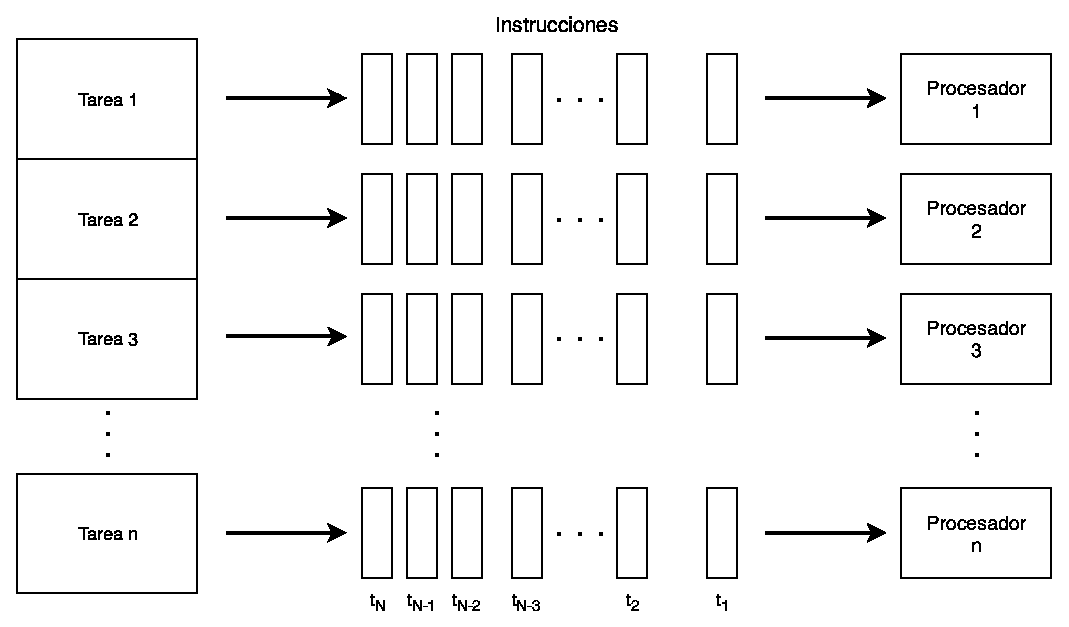
\includegraphics[width=0.8\textwidth]{parallel_figure}
   \label{fig:parallel_figure}
 \end{figure}
 
 
 Los ciclos son regiones de c\'odigo potencialmente paralelizables, con excepci\'on de aquellos donde exista dependencia entre iteraciones. 
 
\subsubsection{M\'etricas para evaluar paralelizaci\'on y vectorizaci\'on}
 
Existen m\'etricas para evaluar el comportaminto de los algoritmos y se obtienen por medio de la lectura de registros especializados en el KNL. Estas m\'etricas se pueden obtener gracias al muestreo de estos registros por medio de las herramientas de perfilado. Dichas m\'etricas son \'utiles para identificar las secciones del programa donde las optimizaciones pueden generar un impacto en el tiempo de ejecuci\'on.

El proceso de ajuste del rendimiento del algoritmo pasa por conocer c\'omo se ejecutan las aplicaciones a nivel de los componentes en la arquitectura como \engl{pipelines}, cach\'es, VPU, etc.

Las m\'etricas utilizadas en este trabajo se listan a continuaci\'on:

\paragraph*{Ciclos por instrucci\'on (CPI):}

Esta m\'etrica consiste en el n\'umero promedio de ciclos requeridos por hilo para ejecutar una instrucci\'on y se considera como un indicador de la latencia presente, que afecta el tiempo de ejecuci\'on de una aplicaci\'on.

La m\'etrica CPI promedio por hilo est\'a dada por:
\begin{equation}\label{eq:CPI_metric}
\text{CPI}_{\text{hilo}} = \frac{\text{\# de ticks de reloj}}{\# \text{de instrucciones}}
\end{equation}

Adem\'as, se puede calcular los CPI promedio por CPU como:

\begin{equation}\label{eq:CPIc_metric}
\text{CPI}_{\text{CPU}} = \frac{\text{CPI}_{\text{hilo}}}{\text{cantidad CPU}}
\end{equation}

El valor de $\text{CPI}_{\text{CPU}} $ se reduce al aumentar la cantidad de hilos de ejecuci\'on, por lo tanto, al optimizar se debe conseguir el menor $\text{CPI}_{\text{CPU}} $. Adem\'as, se debe tomar en cuenta que al utilizar instrucciones vectoriales el CPI tiende a aumentar, debido a que la cantidad de trabajo realizado con una s\'ola instrucci\'on aumenta \cite{Jeffers2016315}.

\paragraph*{Uso de VPU}

Esta m\'etrica permite obtener la intensidad en instrucciones vectorizables a raz\'on de las instrucciones escalares, dando una medida de la eficiencia en t\'erminos de opraciones en punto flotante por segundo\cite{Jeffers2016315}. Es\'a definida como:

\begin{equation}
\textrm{VPUi}= \frac{\textrm{\# SIMD empaquetadas}}_{\textrm{\# SIMD empaquetadas}+\textrm{\# SIMD escalares}}
\end{equation}
